\clearpage
\section{Additional Experimental Results}
\label{app:additional-experimental-results}

\subsection{Ancestral Sampling Results}
\label{app:ancestral-sampling-results}
Table~\ref{tab:uniform-ancestral-expanded} reports the detailed Duo$^{\mathrm{a}}$ results corresponding to the main OWT comparison. As mentioned above, Figure~\ref{fig:owt-genppl-steps} shows the corresponding GenPPL and entropy curves together with the other step-scaling results. Under ancestral sampling, IDLM-DCD remains strongest in the aggressive low-step regime. In particular, the 8-step sampler gives the clearest speed-quality tradeoff: it stays close to the 1024-step Duo teacher while reducing the reverse-step budget by $128\times$.

\begin{table}[t]
    \caption{\textbf{Duo$^{\mathrm{a}}$ distillation comparison.} We report GenPPL $\downarrow$, MAUVE $\uparrow$, and Entropy $\uparrow$. Methods are grouped by Steps, with the best metrics bolded in each group.}
    \label{tab:uniform-ancestral-expanded}
    \centering
    \footnotesize
    \setlength{\tabcolsep}{5pt}
    \begin{tabular}{lcccc}
        \toprule
         & {\scriptsize Steps} & {\scriptsize GenPPL $\downarrow$} & {\scriptsize MAUVE $\uparrow$} & {\scriptsize Entropy $\uparrow$} \\
        \midrule
        FLM~\citep{lee2026flow} & \multirow{2}{*}{1024} & \textbf{62.23} & -- & 5.33 \\
        Duo$^{\mathrm{a}}$ (Teacher)~\citep{sahoo2025the} & & 77.69 & \textbf{0.96} $\pm$ 0.01 & \textbf{5.55} \\
        \midrule
        ELF~\citep{hu2026elf} & \multirow{4}{*}{32} & \textbf{24.08} $\pm$ 0.16 & -- & 5.14 \\
        FMLM~\citep{lee2026flow} & & 45.09 & -- & 5.25 \\
        Duo-DCD$^{\mathrm{a}}$~\citep{sahoo2025the} & & 61.31 & \textbf{0.97} $\pm$ 0.01 & \textbf{5.52} \\
        IDLM-DCD$^{\mathrm{a}}$ (\textbf{Ours}) & & 42.13 $\pm$ 3.65 & 0.94 $\pm$ 0.01 & 5.41 $\pm$ 0.05 \\
        \midrule
        ELF~\citep{hu2026elf} & \multirow{4}{*}{16} & \textbf{33.66} $\pm$ 1.09 & -- & 5.16 \\
        FMLM~\citep{lee2026flow} & & 63.63 & -- & 5.29 \\
        Duo-DCD$^{\mathrm{a}}$~\citep{sahoo2025the} & & 75.24 & \textbf{0.96} $\pm$ 0.01 & \textbf{5.53} \\
        IDLM-DCD$^{\mathrm{a}}$ (\textbf{Ours}) & & 52.06 $\pm$ 4.23 & 0.95 $\pm$ 0.01 & 5.44 $\pm$ 0.05 \\
        \midrule
        ELF~\citep{hu2026elf} & \multirow{4}{*}{8} & 67.32 $\pm$ 2.25 & -- & 5.14 \\
        FMLM~\citep{lee2026flow} & & 86.5 & -- & 5.36 \\
        Duo-DCD$^{\mathrm{a}}$~\citep{sahoo2025the} & & 111.88 & 0.94 $\pm$ 0.01 & \textbf{5.52} \\
        IDLM-DCD$^{\mathrm{a}}$ (\textbf{Ours}) & & \textbf{66.41} $\pm$ 4.59 & \textbf{0.95} $\pm$ 0.01 & 5.42 $\pm$ 0.03 \\
        \midrule
        FMLM~\citep{lee2026flow} & \multirow{3}{*}{4} & 111.31 & -- & 5.26 \\
        Duo-DCD$^{\mathrm{a}}$~\citep{sahoo2025the} & & 261.82 & 0.79 $\pm$ 0.02 & \textbf{5.50} \\
        IDLM-DCD$^{\mathrm{a}}$ (\textbf{Ours}) & & \textbf{111.29} $\pm$ 8.39 & \textbf{0.88} $\pm$ 0.02 & 5.32 $\pm$ 0.06 \\
        \bottomrule
    \end{tabular}
\end{table}

The main comparison is with Duo-DCD under the same ancestral sampler. At 8 steps, IDLM-DCD improves GenPPL from 111.88 to 66.41 while keeping MAUVE and entropy close to the teacher. At 4 steps, Duo-DCD degrades sharply, whereas IDLM-DCD still preserves a usable quality-diversity tradeoff. Thus the benefit of IDLM is largest when very few reverse steps must replace the original 1024-step teacher trajectory.

\subsection{\texorpdfstring{GenPPL and Entropy vs. Sampling Steps}{GenPPL and Entropy vs. Sampling Steps}}
\label{app:genppl-step-plots}
Figure~\ref{fig:owt-genppl-steps} provides the main GenPPL and entropy curves that complement the compact OWT summary in Figure~\ref{fig:owt-main-results}. These plots show how generation quality and token-level diversity change as the number of reverse sampling steps is reduced. For MDLM, IDLM-MDLM gives the strongest low-step tradeoff relative to the teacher and SDTT baselines, improving GenPPL while maintaining comparable entropy. For Duo$^{\mathrm{g}}$, IDLM-DCD is most effective in the aggressive low-step regime, reaching strong GenPPL at $4$ steps while preserving competitive entropy. We also include the ancestral Duo curve here, so the greedy and ancestral step trends can be compared in one place.

\begin{figure*}[t]
    \centering
    \begin{subfigure}[t]{0.32\textwidth}
      \centering
      \includegraphics[width=\linewidth]{images/mdlm_2.pdf}
      \caption{MDLM / SDTT}
    \end{subfigure}\hfill
    \begin{subfigure}[t]{0.32\textwidth}
      \centering
      \includegraphics[width=\linewidth]{images/duo_greedy_2.pdf}
      \caption{Duo$^{\mathrm{g}}$}
    \end{subfigure}\hfill
    \begin{subfigure}[t]{0.32\textwidth}
      \centering
      \includegraphics[width=\linewidth]{images/duo_ancestral_2.pdf}
      \caption{Duo$^{\mathrm{a}}$}
    \end{subfigure}
    \caption{\textbf{OWT GenPPL and entropy vs. sampling steps.} Each panel shows how generation quality and diversity change as the reverse sampling budget is reduced. GenPPL measures sample quality, where lower is better, while entropy tracks output diversity, where higher is better. The panels provide a unified comparison of step-scaling behavior for our IDLM-MDLM, IDLM-DCD$^{\mathrm{g}}$, and IDLM-DCD$^{\mathrm{a}}$ models.}
    \label{fig:owt-genppl-steps}
\end{figure*}

\subsection{Scaling to Larger MDLM}
\label{app:mdlm-scaling}
To test whether IDLM's low-step behavior persists beyond the $169$M setting, we distill an $863$M MDLM~\citep{sahoo2024simple} checkpoint from the SDTT~\citep{deschenaux2024beyond} work. This is the most direct larger-scale comparison available because SDTT uses the same model family and provides matched low-step baselines. As shown in Table~\ref{tab:mdlm-scaling}, IDLM-MDLM consistently improves over SDTT at $32$, $16$, and $8$ sampling steps, improving both GenPPL and entropy in the low-step regime. In particular, the $16$-step sampler preserves the $64\times$ reduction from the $1024$-step teacher, indicating that the acceleration behavior observed in the $169$M experiments also extends to the larger-scale regime.

\begin{table}[t]
\centering
\caption{\textbf{Scaling to an 863M MDLM teacher.} We report GenPPL $\downarrow$ and Entropy $\uparrow$.}
\label{tab:mdlm-scaling}
\footnotesize
\begin{tabular}{lccc}
\toprule
Method ($863$M params) & Steps & GenPPL $\downarrow$ & Entropy $\uparrow$ \\
\midrule
MDLM (Teacher)~\citep{sahoo2024simple} & 1024 & 34.99 & 5.24 \\
\midrule
SDTT~\citep{deschenaux2024beyond} & \multirow{2}{*}{32} & 31.16 & 5.12 \\
IDLM-MDLM \textbf{(Ours)} & & \textbf{13.71} $\pm$ 1.70 & \textbf{5.17} $\pm$ 0.10 \\
\midrule
SDTT~\citep{deschenaux2024beyond} & \multirow{2}{*}{16} & 52.13 & 5.20 \\
IDLM-MDLM \textbf{(Ours)} & & \textbf{24.07} $\pm$ 2.13 & \textbf{5.36} $\pm$ 0.04 \\
\midrule
SDTT~\citep{deschenaux2024beyond} & \multirow{2}{*}{8} & 121.51 & 5.25 \\
IDLM-MDLM \textbf{(Ours)} & & \textbf{67.37} $\pm$ 4.11 & \textbf{5.59} $\pm$ 0.03 \\
\bottomrule
\end{tabular}
\end{table}

\clearpage
\subsection{Ablation Study}
\label{app:ablation-results}

This subsection expands the ablations summarized in
Section~\ref{sec:ablation}. We keep the teacher and evaluation setup fixed, so
the comparisons isolate how gradients are passed to the generator and how much
latent stochasticity is available during masked-diffusion sampling.

\noindent\textbf{Beyond the \textsc{subs} parameterization.}
In masked diffusion, the \textsc{subs} parameterization makes the IDLM-MDLM
generator update mask-only: unmasked positions are copied by both the teacher
and fake model, so their contribution cancels. As discussed in
Section~\ref{sec:practical extension of idlm}, this removes the sampled
intermediate token from the generator gradient and behaves like an implicit
stop-gradient through the absorbing transition. We therefore test whether
explicitly differentiating through the intermediate state improves the update.
Let $x_0=G_\theta(\epsilon)$ and let $m$ denote the mask token. The Gumbel
relaxation softens the full categorical draw from $q_t(\cdot\mid x_0)$,
replacing the hard token by
\[
\tilde{x}^{\mathrm{G}}_t
=
\softmax\!\left(
\frac{\log q_t(\cdot\mid G_\theta(\epsilon)) + g}{\tau}
\right),
\qquad
g_i \overset{\mathrm{i.i.d.}}{\sim}\mathrm{Gumbel}(0,1).
\]
Its objective is
\[
\LC_{\mathrm{Gumbel}}(\theta)
=
-\EE_{t,\epsilon,g}
\left\langle
G_\theta(\epsilon),
\log f^*(\tilde{x}^{\mathrm{G}}_t,t)
-
\log \hat f(\tilde{x}^{\mathrm{G}}_t,t)
\right\rangle .
\]
The Argmax relaxation keeps the forward state closer to the hard masked
process by using the Gumbel-max form of
$q_t(x_t\mid x_0)=\alpha_t\delta_{x_0}(x_t)+(1-\alpha_t)\delta_m(x_t)$:
\[
b_{\mathrm{copy}}
=
\mathbf{1}\{\log \alpha_t + g_1
\geq
\log(1-\alpha_t)+g_2\},
\qquad
b_{\mathrm{mask}}=1-b_{\mathrm{copy}},
\]
\[
\tilde{x}^{\mathrm{A}}_t
=
b_{\mathrm{copy}}G_\theta(\epsilon)
+
b_{\mathrm{mask}}m,
\qquad
g_1,g_2 \overset{\mathrm{i.i.d.}}{\sim}\mathrm{Gumbel}(0,1).
\]
The corresponding objective is
\[
\LC_{\mathrm{Argmax}}(\theta)
=
-\EE_{t,\epsilon,g_1,g_2}
\left\langle
G_\theta(\epsilon),
\log f^*(\tilde{x}^{\mathrm{A}}_t,t)
-
\log \hat f(\tilde{x}^{\mathrm{A}}_t,t)
\right\rangle .
\]
Figure~\ref{fig:ablation-masked} shows that this additional gradient path does
not improve the masked-diffusion tradeoff. The \textsc{subs} update reaches the
useful low-GenPPL regime fastest while preserving substantially more entropy
than Argmax. Gumbel is smoother, but it reduces GenPPL more slowly and gives a
weaker quality--diversity profile near the shared training budget. This
supports the main-text hypothesis that feeding soft or branch-switched
intermediate states to an MDLM teacher can move the evaluation outside the
one-hot training domain and weaken the distillation signal.

\begin{center}
    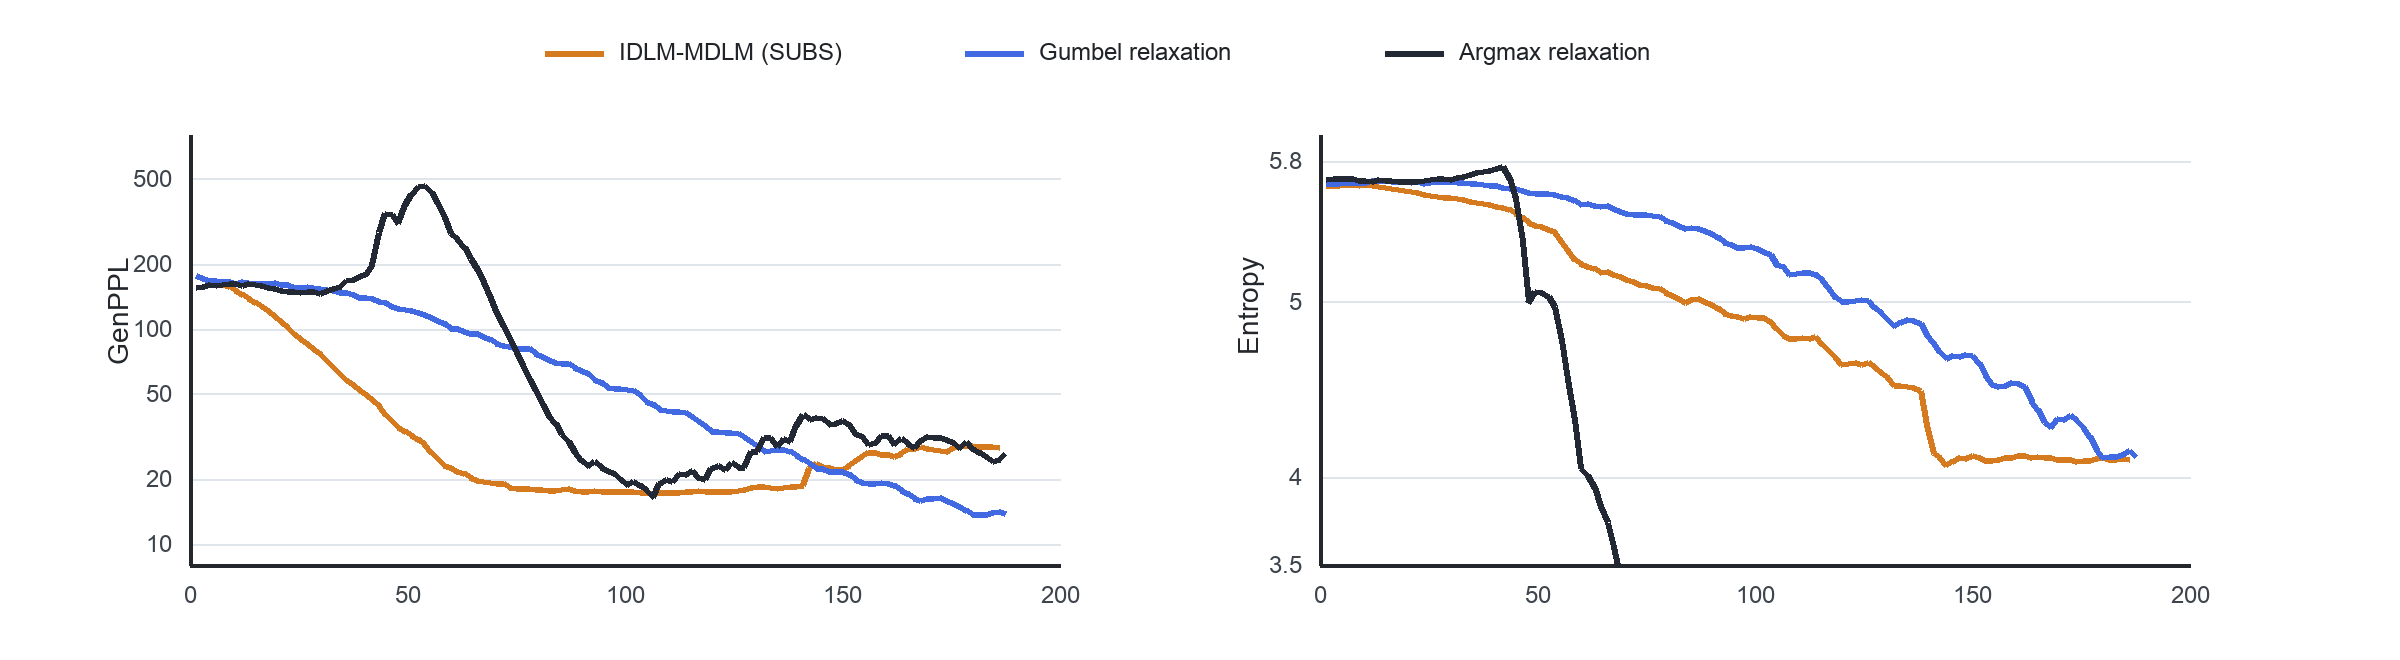
\includegraphics[width=0.98\textwidth]{images/ablation_masked_parameterizations.png}
    \vspace{-0.8em}

    {\small Training steps (k)}
    \captionsetup{hypcap=false}
    \captionof{figure}{
    \textbf{Masked-diffusion parameterization ablation.}
    Validation GenPPL and entropy for IDLM-MDLM with the \textsc{subs},
    Gumbel, and Argmax generator updates. The \textsc{subs} update gives the
    strongest early quality--diversity tradeoff under the shared training
    budget.
    }
    \label{fig:ablation-masked}
\end{center}

\noindent\textbf{DMD-like uniform distillation.}
For uniform diffusion, the Duo parameterization evaluates denoisers on relaxed
states, so the intermediate state remains differentiable. This makes the
difference between full inverse distillation and a DMD-like stop-gradient
reduction directly testable. Let
\[
\begin{aligned}
a_t(w,x)
&= g_{\mathrm{Duo}}\bigl(x_t(w),x,f^*(x_t^\tau(w),t)\bigr)\\
&\quad - g_{\mathrm{Duo}}\bigl(x_t(w),x,f(x_t^\tau(w),t)\bigr),
\end{aligned}
\]
where \(x_t(w)=\argmax(w)\) and \(x_t^\tau(w)=\softmax(w/\tau)\) are the
hard and relaxed Duo states. The full IDLM-Duo objective and the DMD-like
stop-gradient objective use the same teacher--fake Duo advantage, but differ in
whether the relaxed intermediate state carries gradients:
\begin{equation}
\label{eq:uniform-full-vs-sg}
\begin{aligned}
w_t
&= \tilde{\alpha}_t G_\theta(\epsilon)
 + \sqrt{1-\tilde{\alpha}_t^2}\,\xi,\\
w_t^{\mathrm{sg}}
&= \tilde{\alpha}_t \text{sg}\!\left(G_\theta(\epsilon)\right)
 + \sqrt{1-\tilde{\alpha}_t^2}\,\xi,\\
\LC_{\mathrm{IDLM}}^{\mathrm{Duo}}(\theta)
&= \EE\!\left[a_t(w_t,G_\theta(\epsilon))\right],\\
\LC_{\mathrm{DMD\text{-}like}}^{\mathrm{Duo}}(\theta)
&= \EE\!\left[a_t(w_t^{\mathrm{sg}},G_\theta(\epsilon))\right].
\end{aligned}
\end{equation}
Figure~\ref{fig:ablation-uniform} shows that this distinction matters in the
uniform case. The stop-gradient variant quickly enters a high-GenPPL,
high-entropy regime, so its entropy reflects instability rather than useful
diversity. In contrast, the full IDLM-Duo update remains controlled for most of
training. Thus, the formal connection between IDLM and DMD-like matching does
not imply that the two generator updates have the same optimization behavior
for uniform diffusion; the pathwise gradient through the relaxed intermediate
state is empirically important.

\begin{center}
    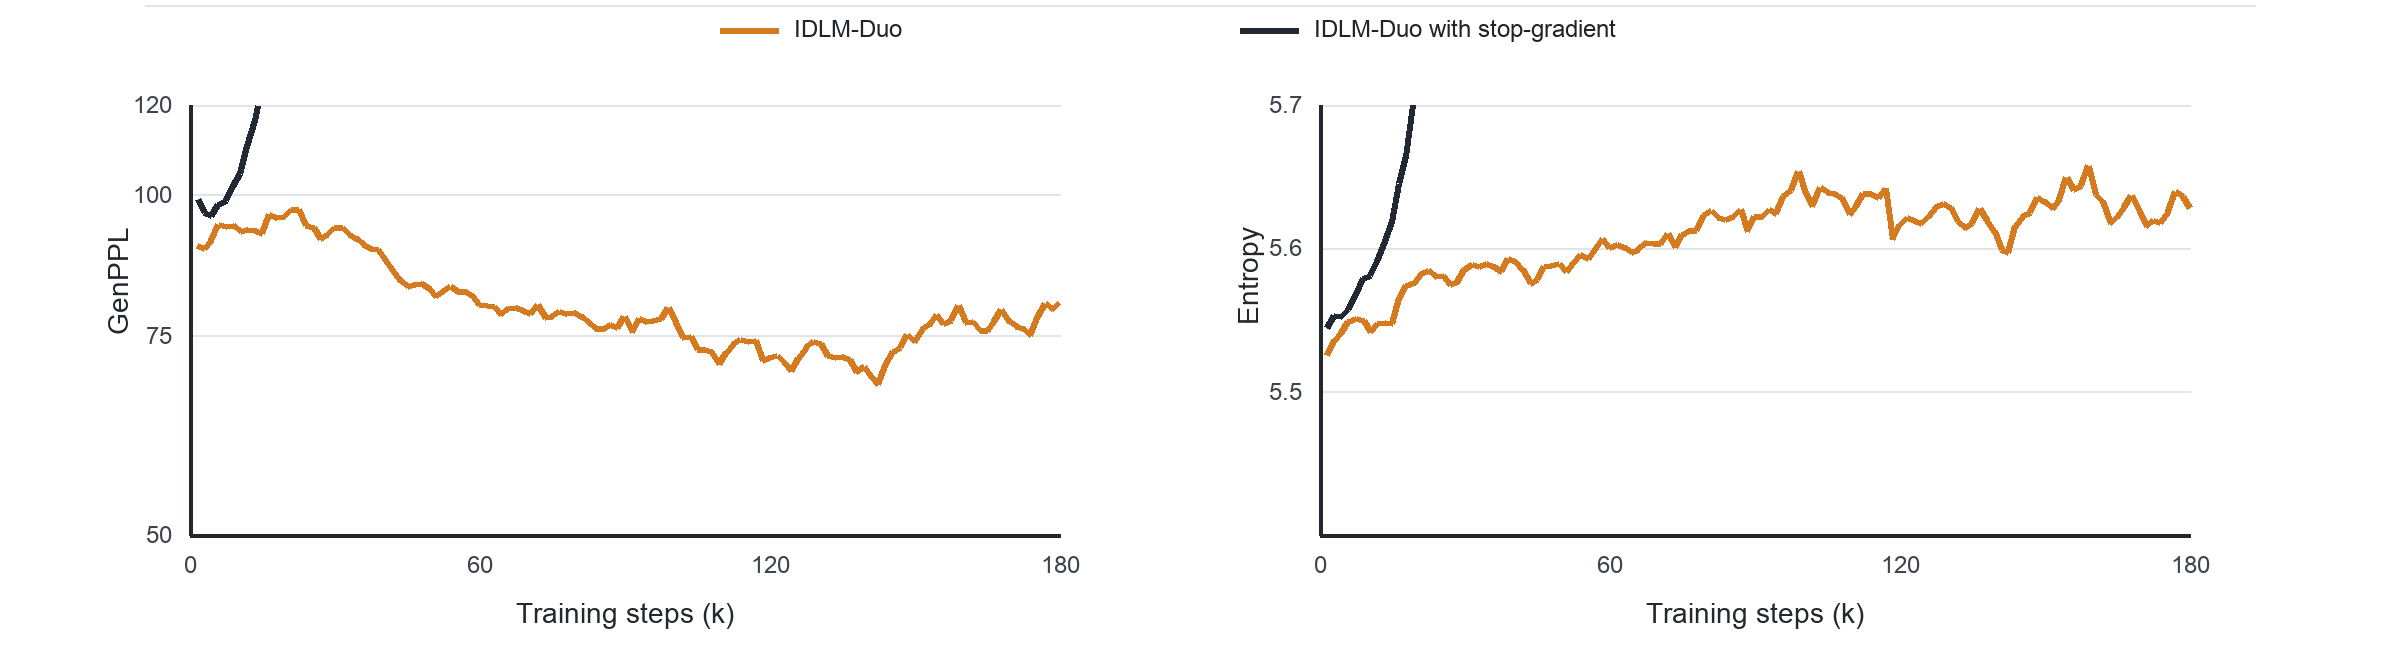
\includegraphics[width=0.98\textwidth]{images/ablation_uniform_stop_gradient.png}
    \captionsetup{hypcap=false}
    \captionof{figure}{
    \textbf{Uniform-diffusion stop-gradient ablation.}
    Validation GenPPL and entropy for IDLM-Duo and its DMD-like
    stop-gradient variant. Removing the intermediate-state gradient leads to a
    divergent high-GenPPL regime, whereas the full IDLM update remains stable.
    }
    \label{fig:ablation-uniform}
\end{center}

\noindent\textbf{Additional latent noise for masked diffusion.}
Finally, we test whether extra latent randomness helps masked diffusion in the
extreme low-step regime. Unlike uniform diffusion, masked diffusion starts from
a deterministic all-mask terminal state, so a deterministic one-step generator
has no rich latent source for sample diversity. We therefore inject Gaussian
noise into the IDLM-MDLM input as a simple control. Table~\ref{tab:gaussian-noise-control}
shows that this modification does not improve GenPPL or entropy:
\begin{center}
    \captionsetup{hypcap=false}
    \captionof{table}{
    \textbf{Additional latent noise for IDLM-MDLM.}
    Values are GenPPL with entropy in parentheses.
    }
    \label{tab:gaussian-noise-control}
    \small
\begin{tabular}{c|cc}
Steps & IDLM-MDLM & IDLM-MDLM + Gaussian noise \\
\hline
1  & 4056.12 (5.87) & 4096.54 (5.88) \\
8  & 79.75 (5.61)  & 81.61 (5.61) \\
16 & 32.75 (5.42)  & 35.76 (5.45) \\
32 & 20.45 (5.23)  & 21.03 (5.26)
\end{tabular}
\end{center}
The negative result is consistent with Section~\ref{sec:ablation}: simple
input-level Gaussian noise is insufficient for masked diffusion, and improving
the low-step regime may require stochasticity that is matched more closely to
the discrete absorbing process.
